\section{Date: 2026-08-04}
\noindent \textbf{Series ID: CPBNDIF066MSFRBPHI} 

\noindent This series is titled Current Physical Plant Capital Expenditures; Diffusion Index for Federal Reserve District 3: Philadelphia and has a frequency of Monthly. The units are Index and the seasonal adjustment is Seasonally Adjusted.The observation start date is 2011-03-01 and the observation end date is 2026-07-01.The popularity of this series is 1. \\ 

\noindent \textbf{Series ID: OCM2MP} 

\noindent This series is titled Real User Cost Index of MSI-M2M (preferred) and has a frequency of Monthly. The units are Percent and the seasonal adjustment is Not Seasonally Adjusted.The observation start date is 1967-01-01 and the observation end date is 2013-12-01.The popularity of this series is 4. \\ 

\subsection{Raw Regression}
\noindent Regresses the two series against each other directly. A significant result here can come just as easily from both series sharing a long-run trend as from any real relationship.

\begin{center}
\begin{tabular}{lclc}
\toprule
\textbf{Dep. Variable:}                  & value\_fred\_OCM2MP & \textbf{  R-squared:         } &     0.001   \\
\textbf{Model:}                          &         OLS         & \textbf{  Adj. R-squared:    } &    -0.031   \\
\textbf{Method:}                         &    Least Squares    & \textbf{  F-statistic:       } &   0.01870   \\
\textbf{Date:}                           &   Tue, 04 Aug 2026  & \textbf{  Prob (F-statistic):} &    0.892    \\
\textbf{Time:}                           &       13:31:41      & \textbf{  Log-Likelihood:    } &    184.86   \\
\textbf{No. Observations:}               &            34       & \textbf{  AIC:               } &    -365.7   \\
\textbf{Df Residuals:}                   &            32       & \textbf{  BIC:               } &    -362.7   \\
\textbf{Df Model:}                       &             1       & \textbf{                     } &             \\
\textbf{Covariance Type:}                &      nonrobust      & \textbf{                     } &             \\
\bottomrule
\end{tabular}
\begin{tabular}{lcccccc}
                                         & \textbf{coef} & \textbf{std err} & \textbf{t} & \textbf{P$> |$t$|$} & \textbf{[0.025} & \textbf{0.975]}  \\
\midrule
\textbf{const}                           &       0.0155  &        0.000     &    36.337  &         0.000        &        0.015    &        0.016     \\
\textbf{value\_fred\_CPBNDIF066MSFRBPHI} &    3.385e-06  &     2.47e-05     &     0.137  &         0.892        &     -4.7e-05    &     5.38e-05     \\
\bottomrule
\end{tabular}
\begin{tabular}{lclc}
\textbf{Omnibus:}       &  9.983 & \textbf{  Durbin-Watson:     } &    0.076  \\
\textbf{Prob(Omnibus):} &  0.007 & \textbf{  Jarque-Bera (JB):  } &    2.548  \\
\textbf{Skew:}          &  0.142 & \textbf{  Prob(JB):          } &    0.280  \\
\textbf{Kurtosis:}      &  1.689 & \textbf{  Cond. No.          } &     39.7  \\
\bottomrule
\end{tabular}
%\caption{OLS Regression Results}
\end{center}

Notes: \newline
 [1] Standard Errors assume that the covariance matrix of the errors is correctly specified.

\begin{figure}
\centering
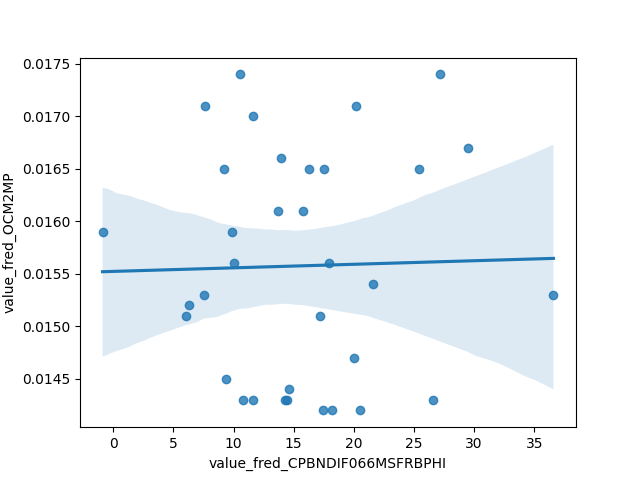
\includegraphics[scale = 0.9]{plots/plot_2026-08-04.png}
\caption{Raw Regression Plot for 2026-08-04}
\end{figure}
\newpage
\subsection{Detrended Regression}
\noindent Regresses the residuals of each series after removing its own linear time trend, so a shared trend can no longer drive the result on its own. A relationship that stays significant here is better evidence of a genuine link between the two series.

\begin{center}
\begin{tabular}{lclc}
\toprule
\textbf{Dep. Variable:}                             & value\_fred\_OCM2MP\_detrended & \textbf{  R-squared:         } &     0.000   \\
\textbf{Model:}                                     &              OLS               & \textbf{  Adj. R-squared:    } &    -0.031   \\
\textbf{Method:}                                    &         Least Squares          & \textbf{  F-statistic:       } &  0.006047   \\
\textbf{Date:}                                      &        Tue, 04 Aug 2026        & \textbf{  Prob (F-statistic):} &    0.939    \\
\textbf{Time:}                                      &            13:31:41            & \textbf{  Log-Likelihood:    } &    193.17   \\
\textbf{No. Observations:}                          &                 34             & \textbf{  AIC:               } &    -382.3   \\
\textbf{Df Residuals:}                              &                 32             & \textbf{  BIC:               } &    -379.3   \\
\textbf{Df Model:}                                  &                  1             & \textbf{                     } &             \\
\textbf{Covariance Type:}                           &           nonrobust            & \textbf{                     } &             \\
\bottomrule
\end{tabular}
\begin{tabular}{lcccccc}
                                                    & \textbf{coef} & \textbf{std err} & \textbf{t} & \textbf{P$> |$t$|$} & \textbf{[0.025} & \textbf{0.975]}  \\
\midrule
\textbf{const}                                      &    4.858e-15  &        0.000     &  3.33e-11  &         1.000        &       -0.000    &        0.000     \\
\textbf{value\_fred\_CPBNDIF066MSFRBPHI\_detrended} &    1.508e-06  &     1.94e-05     &     0.078  &         0.939        &     -3.8e-05    &      4.1e-05     \\
\bottomrule
\end{tabular}
\begin{tabular}{lclc}
\textbf{Omnibus:}       & 10.150 & \textbf{  Durbin-Watson:     } &    0.122  \\
\textbf{Prob(Omnibus):} &  0.006 & \textbf{  Jarque-Bera (JB):  } &    2.467  \\
\textbf{Skew:}          &  0.016 & \textbf{  Prob(JB):          } &    0.291  \\
\textbf{Kurtosis:}      &  1.681 & \textbf{  Cond. No.          } &     7.52  \\
\bottomrule
\end{tabular}
%\caption{OLS Regression Results}
\end{center}

Notes: \newline
 [1] Standard Errors assume that the covariance matrix of the errors is correctly specified.

\begin{figure}
\centering
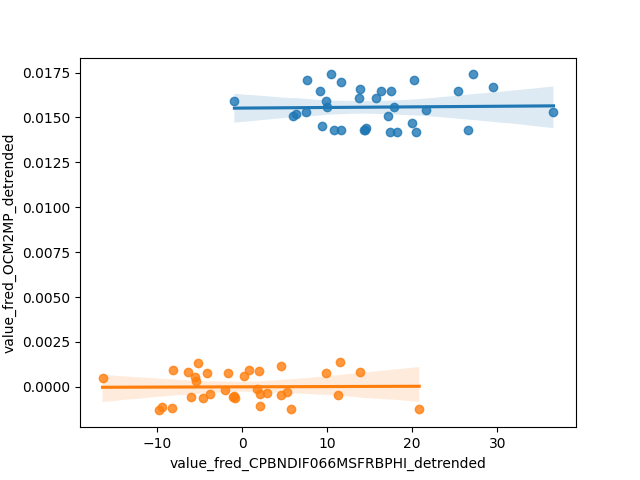
\includegraphics[scale = 0.9]{plots/plot_2026-08-04_detrended.png}
\caption{Detrended Regression Plot for 2026-08-04}
\end{figure}
\newpage
